\documentclass[tikz,border=12pt]{standalone}
\usepackage[utf8]{inputenc}
\usepackage{tikz}
\usetikzlibrary{shapes,arrows.meta,positioning,calc}

\definecolor{ScoutGreen}{HTML}{005432}
\definecolor{ScoutNavy}{HTML}{002855}
\definecolor{ScoutBlue}{HTML}{006EB6}
\definecolor{ScoutRed}{HTML}{A31920}
\definecolor{ScoutAmber}{HTML}{D97706}
\definecolor{BorderGray}{HTML}{CBD5E1}

\begin{document}
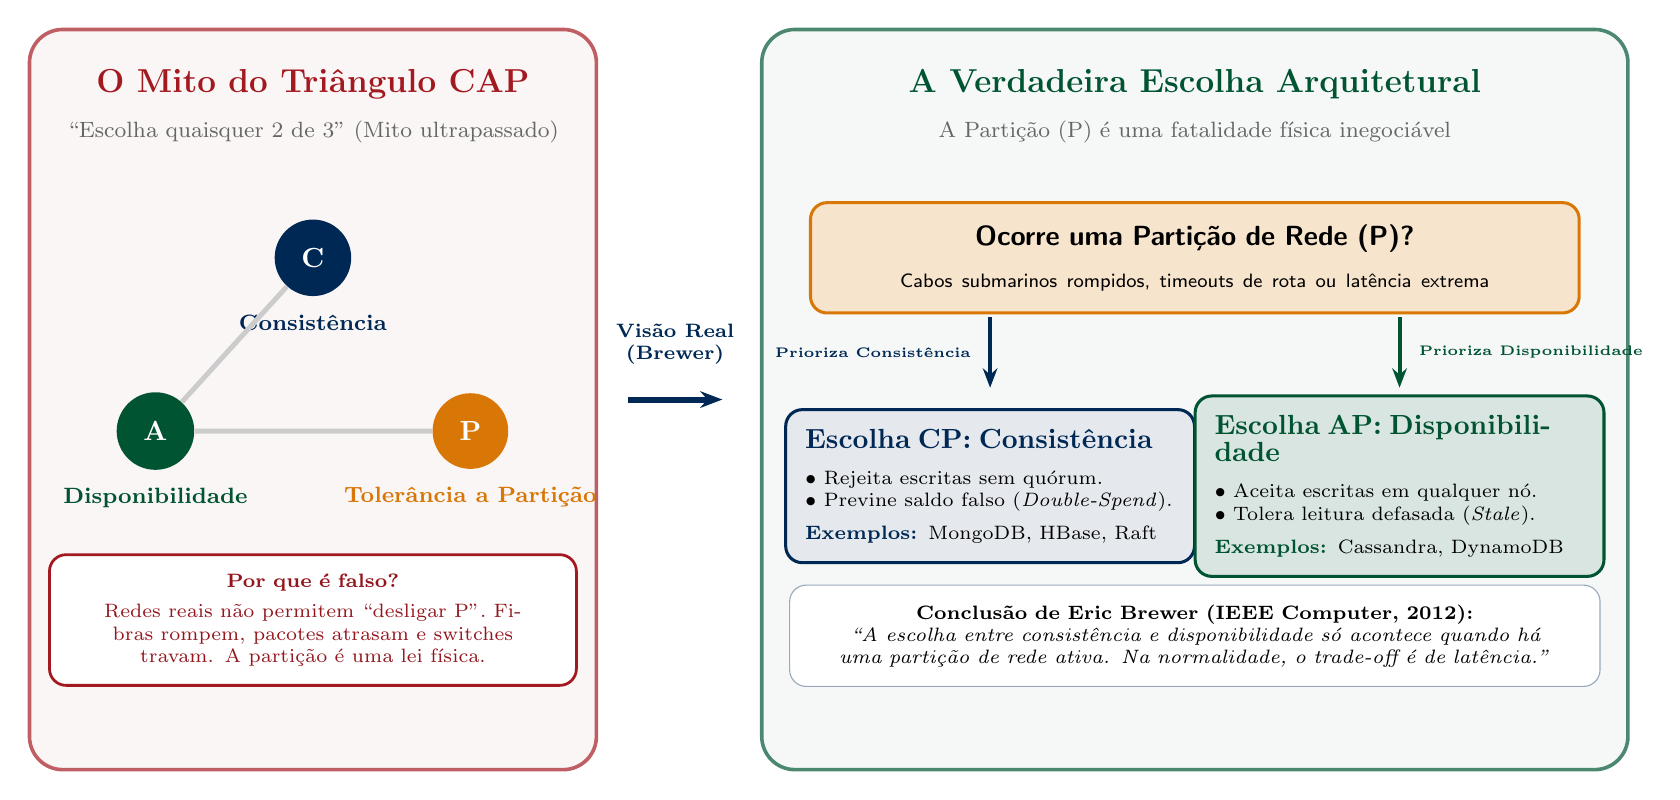
\begin{tikzpicture}[
    font=\sffamily,
    box/.style={draw=BorderGray, rounded corners=6pt, fill=white, line width=1.1pt, align=center, inner sep=6pt},
    arrow/.style={-{Stealth[length=7pt]}, line width=1.4pt}
]

  % =========================================================================
  % PAINEL ESQUERDO: O MITO POPULAR
  % =========================================================================
  \node[draw=ScoutRed!70, rounded corners=12pt, fill=ScoutRed!4, line width=1.3pt, minimum width=7.2cm, minimum height=9.4cm] (p_mito) at (3.6, 0) {};
  
  \node[font=\bfseries\large, text=ScoutRed] at (3.6, 4.0) {O Mito do Triângulo CAP};
  \node[font=\footnotesize, text=gray!80!black] at (3.6, 3.4) {``Escolha quaisquer 2 de 3'' (Mito ultrapassado)};

  % Triângulo
  \node[circle, fill=ScoutNavy, text=white, font=\bfseries\normalsize, inner sep=6pt] (t_c) at (3.6, 1.8) {C};
  \node[font=\footnotesize\bfseries, text=ScoutNavy, below=3pt of t_c] {Consistência};

  \node[circle, fill=ScoutGreen, text=white, font=\bfseries\normalsize, inner sep=6pt] (t_a) at (1.6, -0.4) {A};
  \node[font=\footnotesize\bfseries, text=ScoutGreen, below=3pt of t_a] {Disponibilidade};

  \node[circle, fill=ScoutAmber, text=white, font=\bfseries\normalsize, inner sep=6pt] (t_p) at (5.6, -0.4) {P};
  \node[font=\footnotesize\bfseries, text=ScoutAmber, below=3pt of t_p] {Tolerância a Partição};

  \draw[line width=1.8pt, color=gray!40] (t_c) -- (t_a) -- (t_p) -- cycle;

  \node[draw=ScoutRed, fill=white, rounded corners=6pt, font=\scriptsize, align=center, text=ScoutRed!90!black, line width=1pt, text width=6.2cm, inner sep=7pt] at (3.6, -2.8) {
    \textbf{Por que é falso?}\\[3pt]
    Redes reais não permitem ``desligar P''. Fibras rompem, pacotes atrasam e switches travam. A partição é uma lei física.
  };

  % =========================================================================
  % TRANSIÇÃO CENTRAL
  % =========================================================================
  \draw[-{Stealth[length=8pt]}, line width=2.2pt, color=ScoutNavy] (7.6, 0) -- (8.8, 0);
  \node[font=\scriptsize\bfseries, text=ScoutNavy, align=center] at (8.2, 0.7) {Visão Real\\(Brewer)};

  % =========================================================================
  % PAINEL DIREITO: A REALIDADE ARQUITETURAL
  % =========================================================================
  \node[draw=ScoutGreen!70, rounded corners=12pt, fill=ScoutGreen!4, line width=1.3pt, minimum width=11.0cm, minimum height=9.4cm] (p_real) at (14.8, 0) {};

  \node[font=\bfseries\large, text=ScoutGreen] at (14.8, 4.0) {A Verdadeira Escolha Arquitetural};
  \node[font=\footnotesize, text=gray!80!black] at (14.8, 3.4) {A Partição (P) é uma fatalidade física inegociável};

  % Pergunta Principal
  \node[box, fill=ScoutAmber!20, draw=ScoutAmber, text width=9.2cm, inner sep=8pt] (n_part) at (14.8, 1.8) {
    \textbf{\normalsize Ocorre uma Partição de Rede (P)?}\\[3pt]
    {\scriptsize Cabos submarinos rompidos, timeouts de rota ou latência extrema}
  };

  % Seta para CP
  \draw[arrow, color=ScoutNavy] (12.2, 1.05) -- (12.2, 0.15) node[midway, left=3pt, font=\tiny\bfseries, text=ScoutNavy] {Prioriza Consistência};

  % Seta para AP
  \draw[arrow, color=ScoutGreen] (17.4, 1.05) -- (17.4, 0.15) node[midway, right=3pt, font=\tiny\bfseries, text=ScoutGreen] {Prioriza Disponibilidade};

  % Caixa CP
  \node[box, fill=ScoutNavy!10, draw=ScoutNavy, text width=4.7cm, font=\scriptsize, align=left, inner sep=7pt] (n_cp) at (12.2, -1.1) {
    \textbf{\color{ScoutNavy}\normalsize Escolha CP: Consistência}\\[5pt]
    $\bullet$ Rejeita escritas sem quórum.\\
    $\bullet$ Previne saldo falso (\textit{Double-Spend}).\\[4pt]
    \textbf{\color{ScoutNavy}Exemplos:} MongoDB, HBase, Raft
  };

  % Caixa AP
  \node[box, fill=ScoutGreen!15, draw=ScoutGreen, text width=4.7cm, font=\scriptsize, align=left, inner sep=7pt] (n_ap) at (17.4, -1.1) {
    \textbf{\color{ScoutGreen}\normalsize Escolha AP: Disponibilidade}\\[5pt]
    $\bullet$ Aceita escritas em qualquer nó.\\
    $\bullet$ Tolera leitura defasada (\textit{Stale}).\\[4pt]
    \textbf{\color{ScoutGreen}Exemplos:} Cassandra, DynamoDB
  };

  % Caixa inferior de conclusão
  \node[draw=ScoutNavy!40, fill=white, rounded corners=6pt, font=\scriptsize, align=center, text width=9.8cm, inner sep=7pt] at (14.8, -3.0) {
    \textbf{Conclusão de Eric Brewer (IEEE Computer, 2012):}\\
    \textit{``A escolha entre consistência e disponibilidade só acontece quando há uma partição de rede ativa. Na normalidade, o trade-off é de latência.''}
  };

\end{tikzpicture}
\end{document}
